\chapter{绪论}
\label{ch:introduction}

% 宇宙中可见的物质含量不足以解释所观测到的星系内部以及星系之间彼此产生的引力强度。这就导致了科学家猜测宇宙中有含量多达90%的物质都属于不会辐射电磁波也不会与普通重子物质相互作用的暗物质。
在宇宙学中,暗物质(Dark Matter)是指无法通过电磁波的观测进行研究,也就是不参与电磁相互作用的一类物质形式。
虽然暗物质的属性还不是很明确,但暗物质具有引力相互作用,能够干扰星体发出的光波,从而影响宇宙大尺度结构,因此大量的天文观测结果已经证明了暗物质的存在。
如今,暗物质假说被大多数天文学家所接受,并在大爆炸宇宙学模型,星系的形成与演化模型以及对宇宙微波背景辐射各向异性的解释中扮演重要角色。

最新的研究结果表明\cite{planck_collaboration_planck_2014},宇宙的能量物质组成中\SI{68.3}{\percent}是暗能量,\SI{26.8}是暗物质,而普通物质只占\SI{4.9}{\percent}。这意味着,暗物质在宇宙全部质量中占据了\SI{84.5}{\percent},远远超过了能够被“看到”的普通物质含量。
然而,人们对这部分占主导地位的宇宙成分的理解还仅仅来自于宇宙大尺度结构的观测结果,而对暗物质的组成成分以及性质这类更加细致的问题还知之甚少。
现有的理论模型也不能对暗物质的属性问题给出很好的解释,特别的,在粒子物理学中成功解释了大部分实验结果并给出过精确预言的标准模型(Standard Model)并不包含一个可行的暗物质候选粒子方案,即在标准模型中找不到符合所有已知的暗物质性质的粒子类型。
暗物质这种不能够被现有理论解释的新现象大大激发了科学家们的研究兴趣,它和暗能量一起被称为是笼罩着21世纪物理学的两朵“乌云”。
暗物质粒子探测是当前的科学热点, 具有重要的物理意义和前景, 世界各国都在集中人力、物力和财力研究这一问题。
就像一个多世纪前的两朵“乌云”催生了现代物理学的基础:量子力学和相对论一样,对暗物质粒子的探测和研究很可能导致物理学产生新的革命。

随着科学技术的进步,近年来对暗物质的探测研究渐渐向精确测量方向发展。
暗物质粒子探测卫星(DArk Matter Particle Explorer,简称DAMPE)是中国科学家独立提出并自主研制的空间暗物质探测项目,它于2015年12月24日成功发射并进入预定轨道。
DAMPE是目前世界上观测能段范围最宽、能量分辨率最优的空间暗物质粒子探测器,它的成功发射不仅标志着我国在空间暗物质探测领域占有了一席之地,而且将为今后的暗物质研究提供更多新的有价值的观测数据,为解决暗物质之迷提供助力。

\section{暗物质研究的现状}
\subsection{暗物质存在的证据:宇宙大尺度结构的观测结果}
暗物质的存在已经被各个宇宙学尺度的天文观测结果所证实。
下面依次从星系尺度范围(Galactic Scale),星系团尺度范围(The Scale of Galaxy Clusters)和宇宙尺度范围(Cosmological Scale)三个方面,对一些能够证明暗物质存在的典型证据进行介绍。

在星系尺度范围,暗物质存在最令人信服和直接的证据来自于星系旋转曲线或(Galaxy Rotation Curve,也叫作星系自转曲线)的观测结果。
星系旋转曲线是指星系中的恒星或气体的轨道速度$V(r)$与它们距离星系中心的距离$r$之间的关系曲线。
根据开普勒定律,在距离星系质量中心区域很远的恒星或气体,其轨道速度应该满足$V(r)\propto 1/\sqrt{r}$,即距离星系中心的越远,它们的轨道速度就越小;
而对大量旋转星系的观测\cite{rubin1980rotational}却发现,其内部星体的轨道速度并没有出现预期的随距离平方根减小,而是表现得较为平坦,如图\ref{fig:introduction:rotation_curve}所示。
\begin{figure}[htbp]
	\centering
	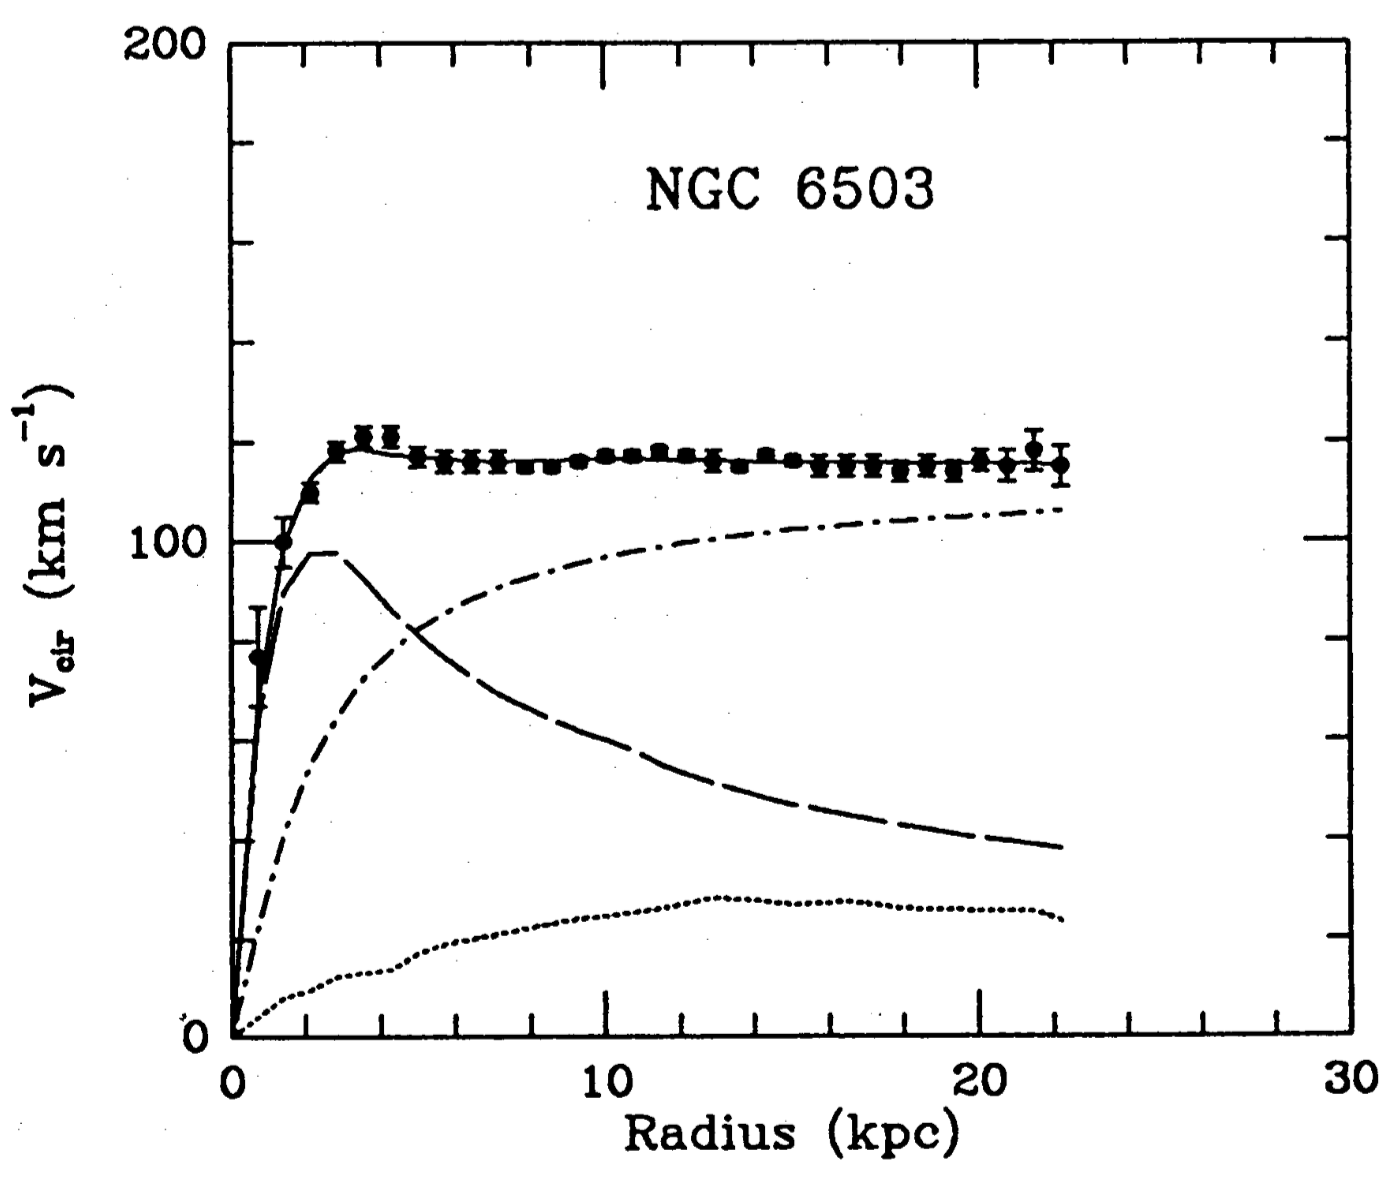
\includegraphics[width=0.65\textwidth]{chap/introduction/fig/rotation_curve.png}
	\caption{一个典型的星系旋转曲线,引自\cite{begeman_extended_1991}。其中黑色方块是观测值,虚线代表可见物质的贡献,点线代表气体的贡献,点虚线是暗物质晕(dark matter halo)的贡献,而实现是三种成分的组合。}
	\label{fig:introduction:rotation_curve}
\end{figure}
这个现象表明,星系内部存在大量的“不可见”物质:暗物质晕,它们弥漫在星系可见质量中心的周围,并通过引力作用拉住星系外侧的组成,以使其不致因过大的离心力而脱离星系\cite{bosma1978distribution}。
星系旋转曲线的异常现象使得“暗物质”这个概念被科学界普遍接受。

实际上,现代意义上的“暗物质”概念由瑞士天文学家F.Zwicky在1933年研究星系团内的星系运动时首次提出来的\cite{zwicky1933spectral}。
Zwichy根据测得的Coma星系团内星系运动的速度弥散(Velocity Dispersion),应用维里定理得到了该星系团的质光比(Mass-to-light Ratio),发现它比太阳附近的质光比要大两个量级,即Coma星系团内可见部分的质量只占根据万有引力效应测得的星系团总质量的一小部分。
据此,Zwichy认为存在着未被人们观测到的质量缺失,他将这些缺失的质量称之为“暗物质”,然而这在当时并没有引起人们的重视。
如今,有许多办法可以测定星系团的质量,如通过弱引力透镜效应,通过测团内热气体的X射线发射轮廓图以及通过测量径向速度分布等。
特别的,2006年,美國天文学家利用钱德拉X射线望远无意间观测到了Bullet星系团的碰撞过程\cite{bullet_cluster},得到了迄今为止能偶证明暗物质存在的最直接证据。
Bullet星系团由两个碰撞中的星系团组成,
\begin{figure}[htbp]
	\centering
	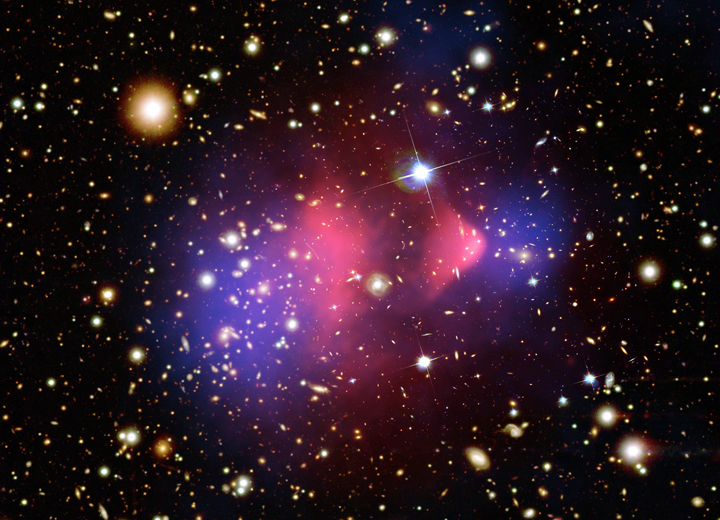
\includegraphics[width=0.65\textwidth]{chap/introduction/fig/bullet_cluster.jpg}
	\caption{Bullet星系团的碰撞过程,其中}
	\label{fig:introduction:bullet_cluster}
\end{figure}
\subsection{暗物质的粒子属性:标准模型之外的物理}
暗物质的性质与组成
现有模型的拓展:SUSY supersymmetry 有暗物质候选粒子


\subsection{暗物质粒子的探测:精细测量时代的到来}
暗物质粒子探测是当前的科学热点, 具有重要的物理意义和前景, 世界各国都在集中人力、物力和财力研究这一问题。根据目前的技术手段, 探测暗物质粒子的方法大致可以总结为三类: 加速器直接产生法,直接探测法和间接探测法。

加速器直接产生法是发现新粒子最常用和最有效的方法。
利用加速器将粒子加速到高能量进行对撞可以模拟宇宙大爆炸初期环境, 各种新的粒子能够在对撞后产生, 其中也可能包含暗物质候选粒子。
通过对次级粒子的探测或逃逸能量(missing energy)的重建, 可以反推出新粒子的存在并在实验室环境下研究粒子的物理特性。
产生暗物质粒子需要极高的能量, 目前只有欧洲核子中心的大型强子对撞机(LHC)能够满足这个条件。
然而, LHC只能产生较轻的暗物质粒子候选粒子, 对于更重的暗物质候选粒子, 需要建造更高能量的加速器和更加强大的粒子探测器。

第二种是直接探测暗物质粒子。该方法是直接探测来自宇宙空间的暗物质粒子与(探测器上的)原子核碰撞所产生的信号。

第三种间接探测暗物质粒子。间接法是观测暗物质粒子在接近银河系中心处发生衰变或相互作用之后产生的稳定粒子如伽玛射线、正电子、反质子、中微子等。

\section{暗物质粒子的空间探测}
\subsection{空间探测的优势}

\subsection{国际上的研究现状}

\section{暗物质粒子探测卫星简介}
暗物质粒子子探测卫星 (英文: DArk Matter Particle Explorer, 缩写: DAMPE)是中国科学院首批空间科学战略先导专项之一, 预计于2015年11月在酒泉卫星发射基地由长征二号丁运载火箭发射上空。
DAMPE粒子探测器是暗物质粒子探测卫星的主要载荷, 它是一个高精度宽能段的能谱探测器,专门用来测量空间中高能电子、高能伽玛射线和重离子的能谱和分布。
一旦成功发射, DAMPE粒子探测器将弥补我国在空间暗物质探测上的空白, 同时也将成为世界上覆盖能区最广,精度最高的空间粒子探测器之一。

\subsection{科学目标}
暗物质粒子探测卫星的科学目标可以归结为以下三个方面:
\begin{enumerate}
	\item 寻找暗物质粒子存在的证据, 这是项目的首要目标。 通过在空间高分辨、宽能段地观测高能电子和伽玛射线寻找和研究暗物质粒子,间接测定其质量、湮灭截面或者寿命等重要的物理参量,并限定暗物质粒子的空间分布,在暗物质研究这一前沿科学领域取得重大突破。
	\item 宇宙线物理研究。通过测量TeV以上的高能电子能谱来研究宇宙线起源, 通过测量TeV/核子的核素能谱来研究宇宙射线传播和加速机制。
	\item 伽玛射线天文学研究。通过观测高能伽玛射线在伽玛天文方面取得重要成果。
\end{enumerate}

DAMPE使用间接探测法来研究暗物质粒子。
根据已有的观测结果 (见上节), 高分辨观测高能伽玛射线和电子是探测暗物质粒子可能的突破点。
空间中高能电子和伽玛射线的流量与能量成反比, 且比宇宙线本底(主要是质子和氦核)低百倍以上, 因此如何进行本底抑制是能否这种方法成功的关键。

宇宙线的起源、加速传播机制是天文学中一个重要的研究课题。
高能电子在星际中传播时,会与背景光发生逆康普顿散射且受星际磁场的作用发生同步辐射而损失能量,损失能量的速度与电子能量的平方成正比。
能量越高的电子损失能量越快,所以高能电子不能够传播太远,高于1012eV的高能电子其寿命只有105年,传播距离只有1kpc。
地球附近的宇宙高能电子只能来自于附近的高能电子源,因此它被常用于研究宇宙线的起源。。
宇宙线中的高能ce


DAMPE粒子探测器本身是一个高空间分辨和能量分辨的伽玛射线望远镜,其主要观测能段超过了国际上所有空间伽玛射线望远镜,可能会有许多预见不到的科学发现。如质子衰变实验发现了天体中微子,开辟了中微子天文学这一新的科学领域,这样的例子很多。我们期望本项目观测能够发现许多人类未知的“第一次”。

\begin{table}[htb]
	\centering
	\caption{DAMPE与其它同类探测器的性能比较}
	\label{tab:ch1:dampe_comparison}
	\begin{threeparttable}
	\begin{tabulary}{\linewidth}{LCCCC}
		\toprule[1.5pt]
		  & DAMPE & AMS-02 & FERMI-LAT & CALET \\ 
		\midrule[1pt]
		Energy Range (\si{GeV}) & $5\sim10^4$ & $0.1\sim10^3$ & $0.02\sim300$ & $1\sim10^3$ \\ 
		$e/\gamma$ Energy res.@\si{GeV}(\si{\percent}) & 1.5 & 3 & 10 & 2 \\ 
		$e/\gamma$ Angular res.@\si{GeV}(\si{\degree}) & 0.1 & 0.3 & 0.1 & 0.1 \\ 
		$e/p$ Discrimination& $10^5$ & $10^5\sim10^6$ & $10^3$ & $10^5$ \\ 
		Calorimeter thickness($\Psi_0$) & 31 & 17 & 8.6 & 30 \\ 
		Geometric accep.(\si{\meter\squared\steradian}) & 0.4 & 0.09 & 1 & 0.12\tnote{*} \\ 
		\bottomrule[1.5pt] 
	\end{tabulary}
	\begin{tablenotes}
		\item[*] DAMPE
	\end{tablenotes}
	\end{threeparttable}
\end{table}
    
\subsection{性能指标}
DAMPE卫星将运行于\SI{500}{\kilo\meter}的太阳同步轨道,设计寿命大于三年。
卫星观测能段覆盖5GeV-10TeV,能量分辨优于1.5%,超过国际上所有类似探测器。可望在暗物质粒子探测和宇宙线物理这两大科学难题上取得突破!同时更好的研究伽玛射线天文学等相关重要科学问题。
\subsection{DAMPE粒子探测器的组成}
DAMPE粒子探测器由四个子探测器系统组成, 分别是塑闪阵列探测器, 硅迳迹探测器, BGO量能器和中子探测器, 见图\ref{fig:dampe_structure}。
下面分别对各子探测器进行简单的介绍。

BGO量能器(BGO Calorimeter, 简称:BGO)
BGO功能,原理
结构
性能参数
BGO触发系统

塑闪阵列探测器(Plastic Scintillator Array Detector, 简称:PSD)。
PSD不参与触发逻辑
塑闪阵列探测器是DAMPE的关键子探测器之一,它的主要功能有两点:
\begin{enumerate}
	\item 协助BGO量能器区分光子事件和电子事件。
	\item 鉴别入射重离子的种类,作为硅阵列探测器电荷测量的备份。
\end{enumerate}

硅迳迹探测器(Silicon-Tungsten Tracker, 简称:STK)
原理,钨板功能
结构
性能参数

中子探测器(Neutron Detector, 简称:NUD)
结构
原理

\begin{figure}
\centering
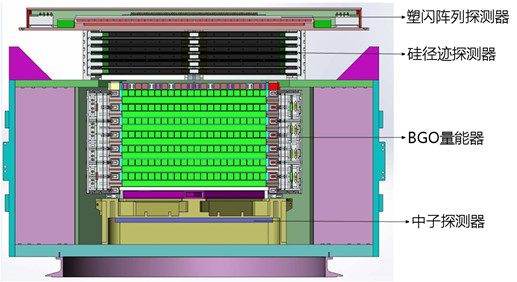
\includegraphics[width=0.8\linewidth]{chap/introduction/fig/dampe_structure_2}
\caption{DAMPE暗物质粒子探测器的整体结构}
\label{fig:dampe_structure}
\end{figure}
